\documentclass[aspectratio=169]{beamer}
\usepackage{amssymb}
\usepackage[utf8]{inputenc}
\usepackage{pifont}% http://ctan.org/pkg/pifont
\usepackage{listings}
\usepackage{minted}
\usepackage[dvipsnames]{xcolor}
\usepackage{tcolorbox}
\usepackage{etoolbox}
\usepackage{caption}
\usepackage{subcaption}
\BeforeBeginEnvironment{minted}{\begin{tcolorbox}}%
\AfterEndEnvironment{minted}{\end{tcolorbox}}%
%\RecustomVerbatimEnvironment{Verbatim}{BVerbatim}{}
\newcommand{\cmark}{\ding{51}}%
\newcommand{\xmark}{\ding{55}}%
\usetheme{Madrid}
\usecolortheme{dolphin}

\newcommand{\pluseq}{\mathrel{{+}{=}}}

\title[Software Optimization for Accelerators] %optional
{Software Optimization for a RISC-V Accelerator}

\subtitle{A case study}

\author[Julien de Castelnau] % (optional)
{Julien de Castelnau}

\date[26-08-2024] % (optional)


\titlegraphic{
\includegraphics[height=0.6cm]{Logo_EPFL.pdf}}

%End of title page configuration block
%------------------------------------------------------------

%------------------------------------------------------------
%The next block of commands puts the table of contents at the 
%beginning of each section and highlights the current section:

%------------------------------------------------------------


\begin{document}

%The next statement creates the title page.
\frame{\titlepage}

%---------------------------------------------------------
\begin{frame}
\frametitle{There's Plenty of Room at the Top... And Plenty of Work Too}
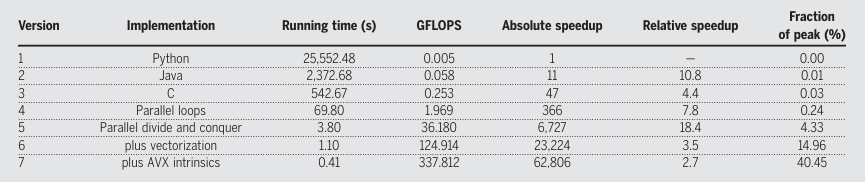
\includegraphics[width=1.0\linewidth]{figs/opt.png}
\begin{itemize}
    \item $\approx$1300x speedup between C versions\pause
    \item Have to repeat for every new HW platform!
    \item \large How do we write software like this for custom hardware?
    %\item How to deal with rapid development of custom hardware?
\end{itemize}
\end{frame}
%---------------------------------------------------------

\begin{frame}[containsverbatim]
\frametitle{Case Study}
\begin{itemize}
\item Hardware: Embedded RISC-V CPU with dense 4x4 matrix multiplication accelerator
\item Programming model:
\begin{itemize}
\item Performs operations on matrices w/ CPU instructions (RISC-V ISE)
\item Matrices stored in special registers $m_0 \dots m_7$
\item E.g. \verb|mmasa.w m2,m0,m1| computes $m_2 \pluseq m_0 \cdot m_1^T$ 
\end{itemize}
\item Software: simplified 1D convolution layer of a CNN (Convolutional Neural Network)
\item Manual optimization process: demo!
\end{itemize}
\end{frame}

\begin{frame}
\frametitle{Background}
\begin{itemize}
\item 1D convolution: Given an input stream $I[I_C][N]$ of length $N$ with $I_C$ input channels, and a array of kernels $K[O_C][I_C][W]$ of width $W$ with $O_C$ output channels, compute output $O[O_C][N]$ s.t.
$$ O[i][j] = \sum_{c = 0}^{I_C} \sum_{r = 0}^{W} \begin{cases} I[c][j+r] \cdot K[i][c][r] & \text{if } j+r<N \\ 0 & \text{otherwise} \end{cases}, 0 \leq i \leq O_C, 0 \leq j \leq N $$\pause
\item Tiled matrix multiplication:

$$X = \begin{bmatrix}
\color{red} x_{0,0}& \color{red} x_{0,1}& \color{blue} x_{0,2}& \color{blue} x_{0,3}\\
\color{red} x_{1,0}& \color{red} x_{1,1}& \color{blue} x_{1,2}& \color{blue} x_{1,3}\\
\color{Green} x_{2,0}& \color{Green} x_{2,1}& \color{YellowOrange} x_{2,2}& \color{YellowOrange} x_{2,3}\\
\color{Green} x_{3,0}& \color{Green} x_{3,1}& \color{YellowOrange} x_{3,2}& \color{YellowOrange} x_{3,3}\\
\end{bmatrix}, Y = \begin{bmatrix}
\color{red} y_{0,0}& \color{red} y_{0,1}& \color{blue} y_{0,2}& \color{blue} y_{0,3}\\
\color{red} y_{1,0}& \color{red} y_{1,1}& \color{blue} y_{1,2}& \color{blue} y_{1,3}\\
\color{Green} y_{2,0}& \color{Green} y_{2,1}& \color{YellowOrange} y_{2,2}& \color{YellowOrange} y_{2,3}\\
\color{Green} y_{3,0}& \color{Green} y_{3,1}& \color{YellowOrange} y_{3,2}& \color{YellowOrange} y_{3,3}\\
    \end{bmatrix}$$
$$ \implies X \cdot Y = \begin{bmatrix}
{\color{red}X_{0,0}}{\color{red}Y_{0,0}} +  {\color{blue}X_{0,1}}{\color{Green}Y_{1,0}} & {\color{red}X_{0,0}}{\color{blue}Y_{0,1}} +  {\color{blue}X_{0,1}}{\color{YellowOrange}Y_{1,1}} \\
{\color{Green}X_{1,0}}{\color{red}Y_{0,0}} +  {\color{YellowOrange}X_{1,1}}{\color{Green}Y_{1,0}} & {\color{Green}X_{1,0}}{\color{blue}Y_{0,1}} +  {\color{YellowOrange}X_{1,1}}{\color{YellowOrange}Y_{1,1}} \\
\end{bmatrix}$$
\end{itemize}
\end{frame}

\begin{frame}
    \frametitle{Summary}
    \begin{itemize}
    \item Performance \large{16x}, but \textit{code length} \large{5x}!
    \item Not shown: time to develop, debug, discard bad ideas..
    \item No longer immediately evident what the program does
    \item Problems worsen as source problem becomes more complex \pause
    \item What if we captured our incremental \textit{refinement} of the code, as code itself?
    \end{itemize}
\end{frame}
    
\begin{frame}
    \frametitle{User-schedulable languages}
    \begin{itemize}
    \item Idea: Separate the algorithm from the way it is carried out - the \textit{schedule} \pause
    \item Programmer optimizes by writing schedule, while preserving semantics of algorithm
    \item Schedule expresssed in code as \textit{incremental rewrites} of algorithm \pause
    \item Many USLs proposed - not a complete literature survey!
    \end{itemize}
\end{frame}

\begin{frame}[containsverbatim]
    \frametitle{TVM}
    \begin{itemize}
    \item End-to-end deep learning compiler with user-schedulable component
    \item Write algorithm in Python-embedded DSL, e.g. matmul:
    \begin{minted}[
    baselinestretch=1.1,
    fontsize=\footnotesize,
    ]{python3}
@T.prim_func
def matmul(A: T.Buffer((N, N), "float32"), 
    B: T.Buffer((N, N),  "float32"),
    C: T.Buffer((N, N), "float32")) -> None:
    for i,j,k in T.grid(N, N, N):
        vi, vj, vk = T.axis.remap("SSR", [i,j,k])
        C[vi, vj] = C[vi, vj] + A[vi, vk] * B[vj, vk]
    \end{minted}
    \item Use Python functions to rewrite programs, forming schedule
    \begin{itemize}
        \item e.g. \verb|reorder_loops()| reorders nested loops, \verb|split()| does tiling
    \end{itemize}
    \item TVM compiler generates C output, fed to LLVM/GCC
    \end{itemize}
\end{frame}

\begin{frame}
    \frametitle{TVM limitations}
    \begin{itemize}
    \item Can't represent HW assembly instructions in TVM IR \pause
    \item Two options:
    \begin{enumerate}
        \item Write an LLVM backend to perform instruction selection
        \item Handwrite an optimized ``microkernel'' abstracting away accelerator details
    \end{enumerate}
    \item Both invisible to schedule: Either forced to defer to compiler or blackbox subroutine \pause
    \item Performance engineer: ``Why should I write a compiler? Why should I use TVM if I have to handwrite C anyway?''\pause
    \item Can we make this code generation a scheduling decision?
    \end{itemize}
\end{frame}

\begin{frame}
    \frametitle{Exo}
    \begin{itemize}
    \item Python DSL compiled to C like TVM, but HW support is \textit{externalized} to user, instead of compiler
    \item Provide \textit{instruction} specification and implementation
    \item Backed by a formal model $\implies$ Every re-write is a correct Exo program
    \item Demo!
    \end{itemize}

\end{frame}

\begin{frame}
    \frametitle{OptiTrust}
    \begin{itemize}
    \item Rewrite C/C++ sources directly using OCaml scripts
    \item Transformations formally backed by separation logic
    \item Supports most of the C spec $\implies$ no artificial limitations due to language?
    \item Demo!
    \end{itemize}
\end{frame}

\begin{frame}
    \frametitle{OptiTrust \& Exo}

    \begin{itemize}
    \item DSL often insufficient (TVM \& Exo), but even the C spec is not enough! (OptiTrust)
    \item Challenging language design problem:
    \begin{itemize}
    \item Need inherently nonstandard custom HW-specific constructs
    \item Expect powerful static analysis to ensure correctness
    \item But also want full expressiveness of C language
    \item While being simple enough to warrant learning!
    \end{itemize}
\end{itemize}
\end{frame}

\begin{frame}
    \frametitle{Conclusion}
    \begin{itemize}
    \item Modern high-performance code:
    \begin{enumerate} 
        \item is time-consuming to write, debug, maintain
        \item must employ every optimization available
        \item necessarily demands a high degree of control over HW, down to assembly
    \end{enumerate}
    \item User-scheduled languages help (1), but repeatedly suffer from (2) and (3)!
    \begin{itemize}
        \item Due to (2), when they fail, or are too cumbersome, they go out the window! \pause
    \end{itemize}
    \begin{block}
        
        USLs must contend with challenging design requirements to be considered for replacing industry-standard handwritten C,C++    
    
    \end{block}
    
    \end{itemize}
\end{frame}

\begin{frame}[plain,c]    
    \begin{center}
    \Huge Thank you!
    \end{center}
\end{frame}
\end{document}